\documentclass[../ECON-281-Notes.tex]{subfiles}
\begin{document}
\chapter{Competitive Market Application}
\begin{Definition}
    {Competitive Free Market}
    No government intervention D and S determines the price.

    It is also the maximum total surplus, the sum of the consumer and producer surplus.
\end{Definition}

\begin{Definition}
    {General Equilibrium Analysis}
    We study what happens not only in the market that is directly affected by the government policy but also what happens to other related markets.
\end{Definition}

\begin{Definition}
    {Partial Equilibrium Analysis} 
    We focus only on the market that is directly affected by the government policy.
\end{Definition}
In this chapter we will only talk about Partial Equilibrium Analysis.


\section{Surplus}
\begin{Definition}
    {Consumer Surplus}
    Is the area above price and below the demand curve.
\end{Definition}

\begin{Definition}
    {Producer Surplus}
    Is the area below price and above the supply curve.
\end{Definition}

\begin{Definition}
    {Total Surplus}
    The sum of consumer surplus and producer surplus.
\end{Definition}
\subsection{Area of surplus formula}

\[
    \text{Area of a rectangle} = b \cdot h
\]
\[
    \text{Area of a triangle} = \frac{b \cdot h}{2}
\]

\section{Price Control}
Price control is where the government set the price.

\subsection{Price Floor}
Is the minimum price like a minimum wage, to help the sellers. 
The price floor is higher than the market price otherwise the price floor is not binding or has no effect. 

\begin{figure}[htbp]
    \centering
    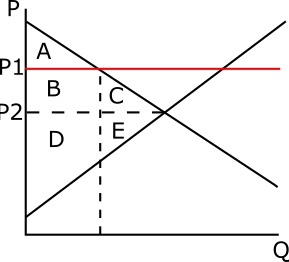
\includegraphics[width=0.8\columnwidth]{../assets/market_floor.png}
    \caption{Market with Price Floor}
    \label{fig:market_floor}
\end{figure}

The quantity traded is at the quantity where the price floor \(P1\)  intersects the demand curve. 

\begin{DndTable}[color=PhbLightGreen]{XXX}
    & \textbf{Before Price Floor} & \textbf{After Price Floor}\\
    C.S & A + B + C & A \\
    P.S & D + E & D + B \\
    D.W.L & None & C + E
\end{DndTable}

\begin{itemize}
    \item \textbf{Consumer} - Worst off he lost area B and C
    \item \textbf{Producer} - Lost E but gained B, could be worst or better off depending on if B or E is bigger. 
\end{itemize}

\newpage
\subsection{Price Ceiling}
Is the maximum price like rent control, to help the consumers.
The price ceiling must be below the market price otherwise the price ceiling is not binding or has no effect.

\begin{figure}[!h]
    \centering
    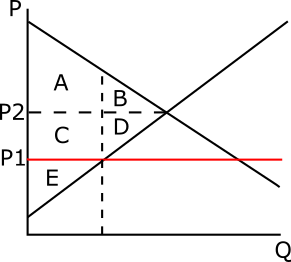
\includegraphics[width=0.8\columnwidth]{../assets/market_ceil.png}
    \caption{Market with Price Ceiling}
    \label{fig:market_ceil}
\end{figure}

The quantity traded is at the quantity where the price ceiling \(P1\)  intersects the supply curve. 

\begin{DndTable}[color=PhbLightGreen]{XXX}
    & \textbf{Before Price Ceiling} & \textbf{After Price Ceiling}\\
    C.S & A + B & A + C \\
    P.S & C + D + E & E \\
    D.W.L & None & B + D
\end{DndTable}
\begin{itemize}
    \item \textbf{Consumer} - lost B but gained C, could be better off or worst off depending on which part is bigger
    \item \textbf{Producer} - Worst off as they lost C and D.
\end{itemize}
    
\section{Production Quota}
The government puts a maximum limit on the produced quantity.

\begin{figure}[!pbth]
    \centering
    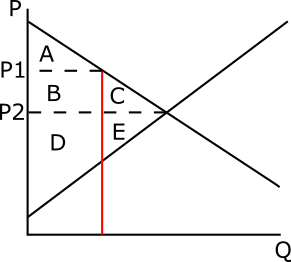
\includegraphics[width=0.8\columnwidth]{../assets/market_quota.png}
    \caption{Market with Production Quota}
    \label{fig:market_quota}
\end{figure}
The price paid by the consumer before the quota was at \(P2\), after the quota the price paid by the consumer is now \(P1\). The amount of quantity traded is the quota amount. 

However, there is a phantom amount of excess supply as the producer wants to produce at price $P1$ but can't because of the quota. So there is an "excess supply" by the amount of goods produced at $P1$ and the amount bought by the consumer at $P1$.

\begin{DndTable}[color=PhbLightGreen]{XXX}
    & \textbf{Before Quota} & \textbf{After Quota}\\
    C.S & A + B + C & A \\
    P.S & D + E & D + B \\
    D.W.L & None & C + E
\end{DndTable}

\begin{itemize}
    \item \textbf{Consumer} - Worst off he lost area B and C
    \item \textbf{Producer} - Lost E but gained B, could be worst or better off depending on if B or E is bigger. 
\end{itemize}

\section{Taxes}
The government can imposes a per unit tax on the producer. This will shift the supply curve to the left by a certain amount. 

In \Cref{fig:market_tax} there is a \$6 dollar tax per unit. The consumer pays \(P^d\) while the producer only receives \(P^s\) or \(P^d - Tax\). 

To find the new supply curve after tax there are two general forms one for Quantity and the other for Price.
\[P = a + bQ + Tax\]
or
\[Q = a + b(P - Tax)\]

\begin{figure}[!pbth]
    \centering
    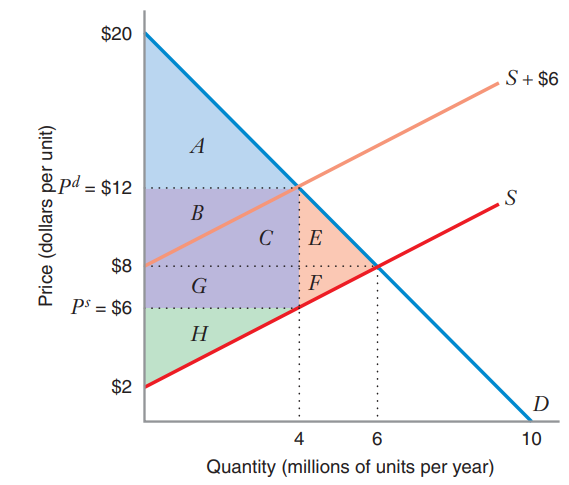
\includegraphics[width=\columnwidth]{../assets/market_tax.png}
    \caption{Market with Tax}
    \label{fig:market_tax}
\end{figure}

\begin{DndTable}[color=PhbLightGreen]{lXXX}
    & \textbf{Before Tax} & \textbf{After Tax} & \textbf{Impact of Tax} \\
    C.S & A + B + C + E &  A  & -B - C - E \\
    P.S & F + G + H & G & -F - G \\
    Gov. revenue & None & B + C + G & B + C + G \\
    D.W.L & None & E + F & E + F
\end{DndTable}

\subsection{Tax incidence}
\begin{Definition}
    {Tax incidence}
    Is how the tax burden is split between the consumer and producer
\end{Definition}


\begin{Definition}
    {Inverse Elasticity rule}
    \[
        \frac{\text{Consumer Share/Burden}}{\text{Producer Share/Burden}} = \frac{\varepsilon_{Q\cdot s, P}}{\varepsilon_{Q \cdot d, P}}  
    \]
\end{Definition}

For \Cref{fig:market_tax} the burdens are:
\begin{itemize}
    \item Consumer's Burden is B + C
    \item Producer's Burden is G
\end{itemize}
When the Inverse Elasticity rule produces a number like 4 it means that the Consumer's Burden is 4 times of the Producer's Burden. 

In general how much burden you pay depends on your elasticity.
The more elastic you are, the less the tax is a burden on you. 
Moreover, the bigger the elasticity, the bigger the DWL. If the elasticity is 0 then the DWL is 0.


\section{Subsidies}
The government can imposes a per unit subsidy on the producer. This will shift the supply curve to the right by a certain amount. 

In \Cref{fig:market_subsidy} there is a \$3 dollar subsidy per unit. The consumer pays \(P^d\) while the producer receives \(P^s\) or \(P^d + Subsidy\). 

To find the new supply curve after the subsidy there are two general forms one for Quantity and the other for Price.
\[P = a + bQ - Subsidy\]
or
\[Q = a + b(P + Subsidy)\]

\begin{figure}[!pbth]
    \centering
    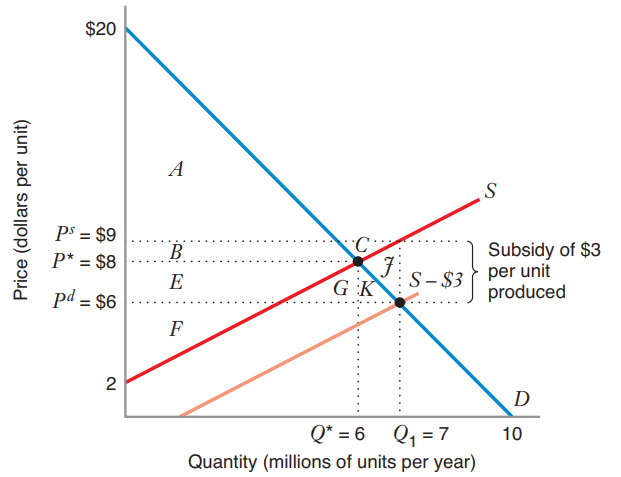
\includegraphics[width=\columnwidth]{../assets/market_sub.png}
    \caption{Market with a Subsidy}
    \label{fig:market_subsidy}
\end{figure}


\begin{DndTable}[color=PhbLightGreen]{lXXX}
    & \textbf{Before Subsidy} & \textbf{After Subsidy} & \textbf{Impact of Subsidy} \\
    C.S & A + B &  A + B + E + G + K & E + G + K \\
    P.S & E + F & B + C + E + F & B + C \\
    Gov. budget & None & -B - C - E - G - K - J & -B - C - E - G - K - J \\
    D.W.L & None & J & J
\end{DndTable}

Like with taxes the more elastic you are the less your share in the subsidy. 

\begin{Note}
    That when we measure the producer surplus after the tax or the subsidy, we use the old supply curve not the new supply curve. 
\end{Note}

\section{Tariff}
The government could impose an import tariff to
\begin{itemize}
    \item Increase the domestic price which allows
    \item Domestic production to increase 
    \item Domestic consumers falls 
    \item imports also falls.
\end{itemize}


\begin{figure}[!pbth]
    \centering
    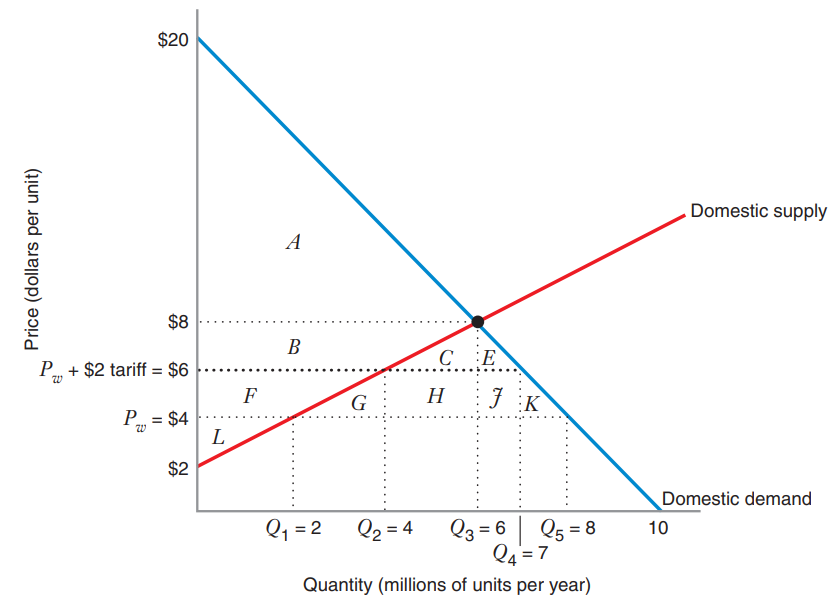
\includegraphics[width=\columnwidth]{../assets/market_tariff.png}
    \caption{Market with Import Tariffs}
    \label{fig:market_tariff}
\end{figure}

\begin{DndTable}[color=PhbLightGreen]{lXXX}
    & \textbf{Before Tariff} & \textbf{After Tariff} & \textbf{Impact of Tariff} \\
    C.S & A + B + C + E + F + G + H + J + K &  A + B + C + E & -F - G - H - J - K \\
    P.S & L & F + L & F \\
    Gov. revenue & None & H + J & H + J \\
    D.W.L & None & G + K & G + K
\end{DndTable}

\begin{Note}
    If the tariff causes the import price to equal the domestic price then this is called a prohibitive tariff. Where import falls to 0 and government tariff revenue falls to 0.
\end{Note}
\end{document}
